% This file was created with tikzplotlib v0.10.1.
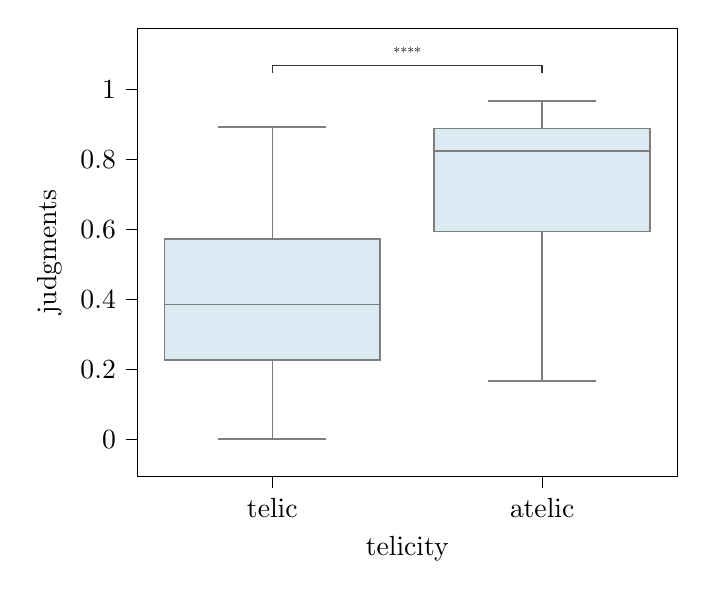
\begin{tikzpicture}

\definecolor{darkgray176}{RGB}{176,176,176}
\definecolor{darkslategray51}{RGB}{51,51,51}
\definecolor{gray127}{RGB}{127,127,127}
% \definecolor{lightgray}{RGB}{211,211,211}
\definecolor{lightgray}{RGB}{219, 234, 242}

\begin{axis}[
tick align=outside,
tick pos=left,
x grid style={darkgray176},
xlabel={telicity},
xmin=-0.5, xmax=1.5,
xtick style={color=black},
xtick={0,1},
xticklabels={telic,atelic},
y grid style={darkgray176},
ylabel={judgments},
% ymin=-0.0483047604397404, ymax=1.01439996923455,
ytick style={color=black}
]
\path [draw=gray127, fill=lightgray, semithick]
(axis cs:-0.4,0.226301802567791)
--(axis cs:0.4,0.226301802567791)
--(axis cs:0.4,0.571274500998456)
--(axis cs:-0.4,0.571274500998456)
--(axis cs:-0.4,0.226301802567791)
--cycle;
\path [draw=gray127, fill=lightgray, semithick]
(axis cs:0.6,0.59342437386382)
--(axis cs:1.4,0.59342437386382)
--(axis cs:1.4,0.887874212042661)
--(axis cs:0.6,0.887874212042661)
--(axis cs:0.6,0.59342437386382)
--cycle;
\addplot [semithick, gray127]
table {%
0 0.226301802567791
0 0
};
\addplot [semithick, gray127]
table {%
0 0.571274500998456
0 0.892011203433431
};
\addplot [semithick, gray127]
table {%
-0.2 0
0.2 0
};
\addplot [semithick, gray127]
table {%
-0.2 0.892011203433431
0.2 0.892011203433431
};
\addplot [semithick, gray127]
table {%
1 0.59342437386382
1 0.1654529478554
};
\addplot [semithick, gray127]
table {%
1 0.887874212042661
1 0.966095208794808
};
\addplot [semithick, gray127]
table {%
0.8 0.1654529478554
1.2 0.1654529478554
};
\addplot [semithick, gray127]
table {%
0.8 0.966095208794808
1.2 0.966095208794808
};
\addplot [semithick, darkslategray51]
table {%
0 1.04628111112478
0 1.06753520571826
1 1.06753520571826
1 1.04628111112478
};
\addplot [semithick, gray127]
table {%
-0.4 0.384423064917596
0.4 0.384423064917596
};
\addplot [semithick, gray127]
table {%
0.6 0.822669634196748
1.4 0.822669634196748
};
\draw (axis cs:0.5,1.06753520571826) ++(0pt,1pt) node[
  scale=0.5,
  anchor=south,
  text=black,
  rotate=0.0
]{****};
\end{axis}

\end{tikzpicture}
